\chapter{Spatial Kappa simulator User Guide}

\section{Obtaining the simulator}

The simulator is available from GitHub as the source Eclipse project, or as a single executable jar file. Both are available at \url{https://github.com/donal-s/SpatialKappa/downloads}. 

\section{Starting the simulator}

\subsection{Running the executable jar}

The simulator can be started by running the executable jar file:\\
\verb|java -jar SpatialKappa-v2.0.6.jar|\\\\
Double clicking the jar file usually works too.

\subsection{Running from the Eclipse project}

The main class of the simulator is \\
\verb|org.demonsoft.spatialkappa.ui.SpatialKappaSimulator|\\\\
Running as a Java Application will bring up the simulator.


\section{Using the simulator}

The initial screen appears as figure \ref{fig:startup}.

\begin{figure}[h!]
 \centering
 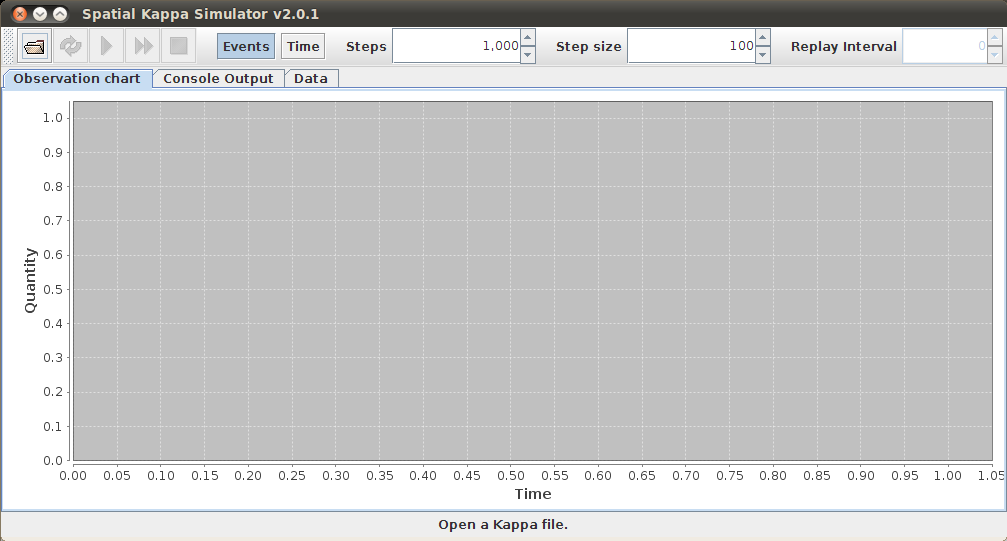
\includegraphics[scale=0.3]{./images/startup.png}
 % startup.png: 1006x510 pixel, 72dpi, 35.49x17.99 cm, bb=0 0 1006 510
 \caption{Initial view}
 \label{fig:startup}
\end{figure}

The toolbar options are:

\begin{tabular}{cl}
 \includegraphics[scale=0.5]{./images/Open.png} & Open a Kappa or Kappa replay file \\
 \includegraphics[scale=0.5]{./images/Reopen.png} & Reopen the current file  \\
 \includegraphics[scale=0.5]{./images/Run.png} & Run the current file \\
 \includegraphics[scale=0.5]{./images/Replay.png} & Replay the current replay file or last run \\
 \includegraphics[scale=0.5]{./images/Stop.png} & Stop the currently running simulation \\
 \includegraphics[scale=0.5]{./images/EventsOrTime.png} & Choose event or time based simulation \\
\end{tabular}

\subsection{Opening a Kappa or Kappa replay file}

Select the 'Open' button on the toolbar and select the file to open. The current implementation expects Kappa source files to have the suffix \verb|.ka| and Kappa replay files (discussed later) to have the suffix \verb|.kareplay|. If the file is parsed successfully, a summary of the Kappa model is displayed in the 'Data' pane (see figure \ref{fig:dataPane}). 

\begin{figure}[h!]
 \centering
 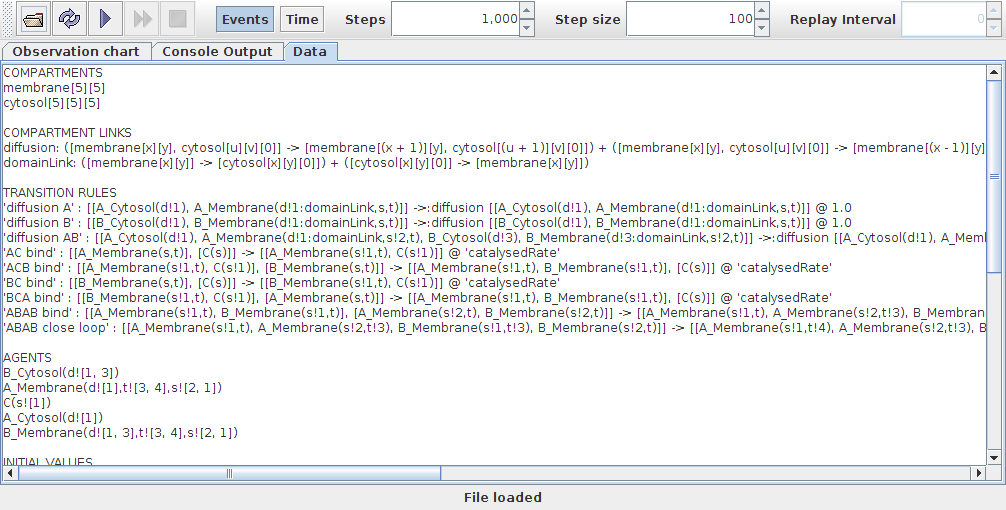
\includegraphics[scale=0.3]{./images/FileOpenDataPane.png}
 % FileOpenDataPane.png: 1006x510 pixel, 72dpi, 35.49x17.99 cm, bb=0 0 1006 510
 \caption{Data pane showing loaded Kappa model}
 \label{fig:dataPane}
\end{figure}

Any errors in reading the Kappa file are shown in the 'Console Output' pane.

The currently open Kappa file can be refreshed from disk by selecting the 'Reopen' button. Useful when editing the Kappa model.

\subsection{Running a simulation}

With a successfully opened Kappa model, one can run a simulation by selecting the 'Run' button. Simulation parameters can be set on the toolbar before running. There is the option to do an event or a time based simulation. For an event based simulation, the number of steps for the simulation (i.e. data points on the time series chart), and the number of finite rate events per step can be set. Equivalent options for time based simulation can also be set.

The simulation can be halted at any point by selecting the 'Stop' button. Note that complex simulations may take some time to start up while data structures are being generated.

A replay file of the simulation is created in the same directory as the Kappa model. The file format is similar to that produced by KaSim.

\subsection{Running a simulation replay}

As the simulation runs, the state of the simulation observables are logged to disk in a replay file after every step. Once the simulation is complete, this replay file can be rerun by selecting the 'Replay' button. The 'Replay Interval' field allows a delay (in ms) to be added between each step.

The file format is similar to that produced by KaSim. Renaming KaSim data output to have the suffix \verb|.kareplay| will allow KaSim output to also be visualised using this tool.

\section{Time series chart}

While the raw data produced from simulations is useful, visualisation of the data is important. There is a simple visualisation panel in the simulator. This is dynamically updated as the simulation runs to give the user an idea of how the simulation is progressing. It is however basic in comparison to some of the commercial simulation data visualisation tools available.

The time series chart is similar to the standard Gnuplot output from KaSim. It is a line graph showing observable quantity against time for all observable definitions in the model. The excellent JFreeChart \citep{JFreeChartwebsite} library was used for generating the charting component. The chart has formatting and save capability, and is zoomable.

\begin{figure}[h!]
 \centering
 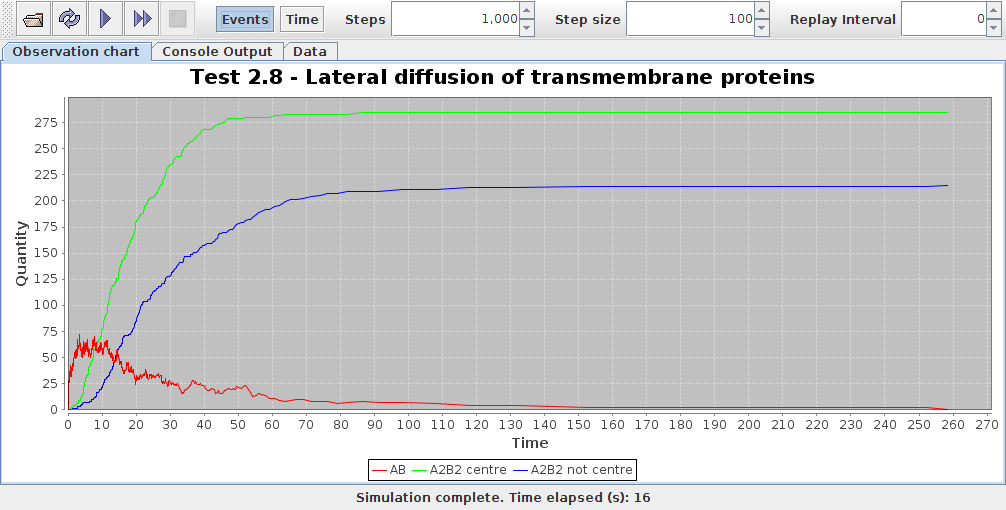
\includegraphics[scale=0.3]{./images/ChartPane.png}
 % ChartPane.png: 1006x510 pixel, 72dpi, 35.49x17.99 cm, bb=0 0 1006 510
 \caption{Sample time series chart output}
 \label{fig:chartPane}
\end{figure}
